\documentclass[output=paper]{langscibook}
\ChapterDOI{10.5281/zenodo.6762274}

\author{Eva Rodríguez-González\affiliation{University of New Mexico} and Marián Giráldez-Elizo\affiliation{Santa Fe Prep High School} and Sarah Schulman\affiliation{New Mexico International School}}
\title{Informing curricular alignment through alternative assessments: The role of learner self-perceptions in Spanish second and heritage language programs}
\abstract{The present quantitative cross-sectional study examines how Spanish language learners in Beginning and Intermediate courses at a university in the U.S. Southwest judge their abilities to organize and perform interpersonal and presentational speaking and writing tasks in the target language. The data set includes self-as\-sess\-ment survey responses from a total of 133 Spanish language learners enrolled in first- and second-year General Education courses. These individuals are matriculated into two different language programs based on their academic or home and/or community exposure to the Spanish language. Participants therefore include Spanish as Second Language learners (SSL, N = 67) and Spanish as Heritage Language Learners (SHL, N = 66). Participants ranged in proficiency from Novice High to Advanced Low and responded to a Can-Do Statement questionnaire (NCSSFL 2014) that was directly aligned to course objectives. Results for the interpersonal speaking and presentational writing domains suggest that participants statistically differed in their self-efficacy based on their language program. In response to this self-efficacy variability, the chapter includes a sample lesson plan that situates inclusivity, equity and diversity as the foundation for all classroom activities. The \textit{Can-Do Statements} are also incorporated to illustrate how conscious awareness of one’s language abilities can foster learner autonomy and inform programmatic assessment.
\keywords{self-efficacy, self-assessment, language learning, speaking, writing, heritage}
}

\IfFileExists{../localcommands.tex}{%hack to check whether this is being compiled as part of a collection or standalone
  \addbibresource{../localbibliography.bib}
  % add all extra packages you need to load to this file

\usepackage{tabularx,multicol}
\usepackage{url}
\usepackage{soul}
\usepackage{longtable, xltabular}
\urlstyle{same}

\usepackage{listings}
\lstset{basicstyle=\ttfamily,tabsize=2,breaklines=true}

\usepackage{langsci-basic}
\usepackage{langsci-optional}
\usepackage{langsci-lgr}

\usepackage{todonotes}

\usepackage{makecell}

\usepackage{enumitem}
\usepackage{multirow}
\usepackage{langsci-branding}
\usepackage{langsci-gb4e}

  \newcommand*{\orcid}{}

\newcommand{\togglepaper}[1][0]{
%   \bibliography{../localbibliography}
    \papernote{\scriptsize\normalfont
    \theauthor.
    \titleTemp.
    To appear in:
    Change Volume Editor \& in localcommands.tex
    Change volume title in localcommands.tex
    Berlin: Language Science Press. [preliminary page numbering]
  }
  \pagenumbering{roman}
  \setcounter{chapter}{#1}
  \addtocounter{chapter}{-1}
}

% \newcommand{\keywords}[1]{\par\textbf{Keywords: #1}}

\renewcommand{\lsChapterFooterSize}{\footnotesize}

  %% hyphenation points for line breaks
%% Normally, automatic hyphenation in LaTeX is very good
%% If a word is mis-hyphenated, add it to this file
%%
%% add information to TeX file before \begin{document} with:
%% %% hyphenation points for line breaks
%% Normally, automatic hyphenation in LaTeX is very good
%% If a word is mis-hyphenated, add it to this file
%%
%% add information to TeX file before \begin{document} with:
%% %% hyphenation points for line breaks
%% Normally, automatic hyphenation in LaTeX is very good
%% If a word is mis-hyphenated, add it to this file
%%
%% add information to TeX file before \begin{document} with:
%% \include{localhyphenation}
\hyphenation{
anaph-o-ra
Dor-drecht
Ku-ka-ma
pre-dom-i-nant-ly
prog-ress
teach-er
Ri-ve-ra
}

\hyphenation{
anaph-o-ra
Dor-drecht
Ku-ka-ma
pre-dom-i-nant-ly
prog-ress
teach-er
Ri-ve-ra
}

\hyphenation{
anaph-o-ra
Dor-drecht
Ku-ka-ma
pre-dom-i-nant-ly
prog-ress
teach-er
Ri-ve-ra
}

  %\togglepaper[]
}{}


\lehead{E. Rodríguez-González, M. Giráldez-Elizo \& S. Schulman}
\shorttitlerunninghead{Informing curricular alignment through alternative assessments}
\begin{document}
\shorttitlerunninghead{Informing curricular alignment through alternative assessments}
\maketitle
\lehead{E. Rodríguez-González, M. Giráldez-Elizo \& S. Schulman}
\section{{Introduction}}
\subsection{{Self-assessment via self-efficacy of language learning}}

\begin{sloppypar}
Student self-assessment in language classrooms occurs when learners assess their own performance, and it is primarily used to help students develop specific learning skills they will need for communicative and intercultural competence. This process may assist in making learners more aware and responsible for their own learning process. Learners' self-assessment practices embedded in Higher Education learning via measurement of self-efficacy have become increasingly popular since the early 2000s \citep{PapanthymouDarra2018}. Documenting language development helps learners to: 1) \emph{develop} important meta-cognitive skills that will allow learners to evaluate their own performance 2) \emph{increase} self-awareness through reflective practice 3) \emph{reinforce} the development of critical reviewing skills through peer evaluation, and 4) contribute to learners’ autonomy. That being said, self-assessment via self-efficacy gives learners a greater amount of agency regarding assessment, thus enriching their learning. Skilled self-assessment can be as reliable as other forms of assessment; however, instructors must provide learners with guidance and practice so that the results of these tools closely align with the results from other assessment agencies (e.g. instructors and/or program/degree evaluation).
\end{sloppypar}

In terms of application and measurability of self-efficacy in language classrooms that emphasize meaningful, communicative learning tasks, self-as\-sess\-ment has been recommended as a way to have learners reflect upon their own learning and make judgments of their own performance in the target language \citep{Klein2007}. \textit{LinguaFolio} is a self-monitoring learner portfolio tool that enables goal setting and collection of evidence of language achievement. It was specifically created for measurement of progress and growth in second languages other than English in the context of the U.S. As such, \textit{LinguaFolio} can serve as a type of assessment as it contains a set of multiple language learning standards that have been adapted into classroom goals as “can do” statements that follow the \textit{American Council of Teaching Foreign Languages} (ACTFL) proficiency guidelines. \textit{Can-Do Statements} have been shown to increase learner motivation, language proficiency, and academic achievement (\citealt{CollettSullivan2010}; \citealt{MoellerWu2012}). Although \textit{Can-Do Statements} were originally designed to enhance the learning of second language learners, the same guiding principle can also be applied to heritage learners (\citealt{CoxWinke2018}: 106). The question for educators is how to draw on this information to better respond to the needs of their learners. By identifying learners’ perceived learning abilities, language teachers can better target their instruction to support learners’ developing linguistic proficiency (\citealt[49]{Hlas2018}).

Since the integration of \textit{Can-Do Statements} in second language learner (L2) language classrooms promotes a reflective learning process that is directly correlated with goal setting and self-assessment, language teachers should consider how to provide guidance to learners toward self-regulated and autonomous learning (see \citealt{MoellerYu2015} for a detailed description of \textit{Can-Do Statements}). Given that speaking and writing are often identified by language learners as the most difficult skills to learn, the present study focuses on learners’ self-assessment of their capabilities in these two modalities (\citealt{Aida1994}; \citealt{ChengHorwitzSchallert1999}; \citealt{Phillips1992}).


\subsection{{Self-efficacy: Bandura’s theoretical framework}}

In the context of a language classroom, feeling prepared to communicate verbally in a given situation and being able to engage in a conversation to successfully navigate that situation illustrate the difference between a speaker’s outcome-expectancies and efficacy. The psychological motivation an individual requires to overcome their performance doubts is what \citet{Bandura1977} referred to as \textit{self-efficacy}. To elaborate, self-efficacy concerns “people’s beliefs about their capabilities to produce designated levels of performance that exercise influence over events that affect their lives” (\citealt{Bandura1994}: 2). When an individual believes that they no longer have control over the outcome of a particular event, they may begin to doubt their capabilities. This negative thinking can then culminate in feelings of self-sabotage, lower aspirations, and depression \citep{Weibell2011}. To analyze changes in fearful and avoidant behavior, \citet{Bandura1997} situates self-efficacy as central to his theoretical framework.

As a cognitive process, self-efficacy will vary according to an individual’s lived experiences. \citet{Bandura1997} contends that certain types of self-efficacy can positively influence how individuals approach a given task. These include:

\begin{itemize}
\item[(a)] performance accomplishments or mastery experiences;
\item[(b)] vicarious experiences;
\item[(c)] verbal or social persuasion; and
\item[(d)] physiological, or somatic and emotional, states

(as cited in \citealt[200]{Weibell2011}).
\end{itemize}
Experiences that are self-fulfilling and lead to a sense of accomplishment are most effective at enhancing self-efficacy. Since the application of \citegen{Bandura1986} view of human behavior has been documented for educational contexts, and most particularly, its application to language learning environments \citep{Wenden1998}, Bandura’s theoretical framework plays a pivotal role in the language classroom, as learners are constantly engaging in performance tasks that test the limits of their perceived self-efficacies. As such, self-efficacy in language classrooms is directly related to a learner’s belief or self-assessment about his or her own competence to perform specific tasks (\citealt{Bandura1986}, \citeyear{Bandura1997}). Thus, each learner’s sense of self-efficacy can play a major role in how s/he approaches goals, tasks, and challenges. More importantly, whether learners perceive themselves as capable of doing a given task can predict their performance outcome more often than their real abilities \citep{Bandura1997}.

\subsection{{Self-efficacy in language learning classroom}}

Significant research regarding self-efficacy and other variables in second language learning classrooms, such as learning strategies, performance, and language anxiety, has emerged only within the last few years (\citealt[61]{RaoofiChan2012}). Still missing from these studies is an exploration on how learners’ reported self-efficacies for each specific language skill (i.e. listening, reading, speaking and writing) relate to the modes of communication (i.e. interpretive, presentational and interpersonal) across different learner proficiency levels \citep{TorresTurner2016}. For example, in classrooms where tasks “involve communicative language use in which the user’s attention is focused on meaning rather than grammatical form,” (\citealt[4]{Nunan2004}) learners may perceive some activities in the target language as more challenging than others (e.g., gap filling activity vs. creating a short story in Spanish). Consequently, learners may differ in their reported self-efficacies for completing those tasks \citep{TorresTurner2016}.

\subsection{{Self-efficacy in second language speaking}}

One of the most important variables language educators must consider is how learners’ self-perceived capabilities can impact their performance on a given language task. Furthermore, the nature of the task, whether it is reading, writing, listening, or speaking, will influence a learner’s degree of reported self-efficacy (\citealt{DewaeleFurnham2008}; \citealt{Horwitz2001}; \citealt{Kim2009}; \citealt{MacIntyreClément1997}; \citealt{Phillips1992}; \citealt{RaoofiChan2012}). This aligns with other research regarding how more private tasks, such as reading, elicit lower levels of anxiety, and therefore, result in higher levels of self-efficacy. As such, learners are more objective at evaluating themselves in reading than any of the other language skill, as the privacy allows for learners to escape possible judgement by others (\citealt{MacIntyreClément1997}: 279).

Conversely, speaking tasks have a profound impact on learner self-efficacy, as the absence of privacy tends to produce higher levels of anxiety (\citealt{Ellis1994}; \citealt{HorwitzCope1986}; \citealt{Young1991}; as cited by \citealt{ChengHorwitzSchallert1999}: 418). The fear of making grammar mistakes or mispronunciations in front of others is consistent across all levels of linguistic proficiency (\citealt{Aida1994}; \citealt{MacIntyreClément1997}; \citealt{Phillips1992}). Even learners who are raised in a home where a non-English minority language is spoken may be apprehensive about speaking the target language in front of their peers. They may also feel that their actual performance may not align with classroom expectations.

To illustrate, \citet{Kim2009} studied the anxiety levels of Korean learners of English enrolled in conversational and reading courses and determined that learners enrolled in the more communicative courses experienced higher levels of anxiety because of a “fear of negative evaluation” when speaking spontaneously or in front of others (\citeyear[153]{Kim2009}). When anxiety levels increase, learners are more likely to depreciate their self-efficacy on various learning tasks \citep{MacIntyreClément1997}. However, while a number of empirical studies have focused on the relationship between language learning anxiety in speaking and learner self-efficacy (\citealt{Horwitz2001}; \citealt{HorwitzCope1986}; \citealt{Phillips1992}; \citealt{Woodrow2006}), it is important to note that interpersonal communication tasks also include writing \citep{ChengHorwitzSchallert1999}.

\subsection{{Self-efficacy in foreign language writing}}

While research on writing anxiety is often limited to the study of English as a first language in the U.S., \citet{ChengHorwitzSchallert1999} argue that fear of evaluation can still influence learner performance on a specific writing task. Specifically, the writer’s perceived quality of his encoded message can cause him to doubt his academic writing skills, which may, inadvertently, hinder his career choices (\citealt{DalyMiller1975}; \citealt{DalyShamo1976}). Self-efficacy in speaking and writing tasks are therefore not to be collapsed into similar categories. Rather, writing apprehension is unique to the written domain. As \citet{Woodrow2011} notes, however, “there is relatively little research on the relationship between self-efficacy and writing that elucidates how learners’ perceptions of their abilities influence their performance on written language tasks'' (\citeyear{Woodrow2011}: 511).

To better ascertain this relationship, \citet{Woodrow2011} conducted a study that examined the interplay of learner self-efficacy and anxiety levels when writing in English as a second language. Her results suggested that self-efficacy had a more significant impact on predicting students’ language learning and performance than learners’ feelings of anxiety. However, it is important to note that learners who were more anxious had lower self-efficacies, and consequently, they tended to focus more on the importance of an assessment than the value of their own learning. This fear of failing to meet expectations in oral or written production of a target language was particularly evidenced among learners who were home and community speakers of this language. These heritage language learners added further complexity to understanding and responding to learners’ reported levels of self-efficacy, as their linguistic capabilities varied tremendously.

\subsection{{Self-efficacy in heritage language learners}}

When referencing home and community speakers of the target language, the term \textit{heritage language learner} (HLL) is often used. However, it is important to note that HLL is a widely recognized yet often misunderstood concept. To this day, there is an absence of a definition that fully captures the term’s historical, sociocultural, and psychological complexity. \citet{Valdés2001} provides the most frequently referenced description, explaining that a heritage language learner is “a language student who is raised in a home where a non-English language is spoken, who speaks or at least understands the language, and who is to some degree bilingual in that language and in English” (\citeyear{Valdés2001}: 38). HLLs therefore have diverse range of communicative and cultural experiences, which manifest in linguistic and affective needs that differ from those of traditional second language learners. Examples of the differences between these two learner groups include academic achievement and motivation for enrolling in language courses; these differences are frequently noted in the heritage language literature (\citealt{HedgcockLefkowitz2016}; \citealt{TorresTurner2015}; \citealt{Tallon2009}).

Given the variability of how and when HLLs are exposed to and have acquired some of their language, HLLs often exhibit learning gaps that are not evidenced in second language learners, such as a comprehensive understanding of academic register and metalinguistic knowledge (\citealt{HedgcockLefkowitz2016}; \citealt{TorresTurner2015}). Nonetheless, given that HLLs are typically exposed to the target language at a young age, language educators often assume they will perform equally to or better than L2s on communicative tasks. When HLLs are unable to meet academic register or demonstrate metalinguistic knowledge, this experience can exacerbate deep-seated feelings of inadequacy and frustration (\citealt{CoryellClark2009}; \citealt{Tallon2009}). The pervasive issue, as \citet[2]{HedgcockLefkowitz2016} explain, is that “traditional approaches to foreign language (FL) instruction rarely target the unique educational needs of heritage language (HL) speakers who represent diverse linguistic, cultural, educational, and socioeconomic profiles.” This pedagogical mismatch, in conjunction with the aforementioned factors, is likely leading to lower ratings of self-efficacy on specific language learning tasks that are also experienced by L2 learners.

Empirical studies that focus on the needs and perceptions of HLLs (\citealt{HedgcockLefkowitz2016}; \citealt{TorresTurner2015}; \citealt{Tallon2009}) have found through the use of the \textit{Foreign Language Classroom Anxiety Scale} (FLCAS) that HLLs typically experience greater anxiety with tasks that require reading and writing and less anxiety with those that require speaking. L2s, by contrast, exhibit greater anxiety with more public tasks, such as interpersonal and presentational speaking (\citealt{MacIntyreClément1997}). As previously mentioned, anxiety is an important variable that challenges learners’ self-efficacies. In one study, \citet{Tallon2009} found that self-efficacy ratings among HLLs fluctuated according to the number of complex grammatical structures. That is, the greater the number of language constructs under study, the greater the learners’ level of anxiety. These findings suggest that instruction that helps HLLs capitalize on their current skill set is paramount. It is therefore critical that instructors learn about the language experiences and cultural connections of their heritage students in order to create HLL-specific learning goals and tasks that validate and promote the learners’ home varieties. These goals may include learning specific vocabularies, as well as academic written and spoken registers, that are related to places of employment. By incorporating students’ backgrounds and learning interests into the curriculum, instructors can create a safe space in which HLLs can “share and discuss their language experiences” (\citeyear{Tallon2009}: 125).  Such intentional planning with regards to meaningful learning objectives and activities will help build confidence and increase learner self-efficacies by fostering a sense of community within the classroom. However, more research is needed to understand how HLLs’ self-perceptions of their linguistic and cultural backgrounds influence the way in which they 1) respond to instruction and produce grammatical structures and 2) develop an awareness of and response to their self-reported abilities.

The following study thus explores how L2 and HLLs in two Spanish programs at an institution of higher education in the U.S. Southwest evaluate their capabilities on a variety of  \textit{Can-Do Statements} in the oral and written domains.


\subsection{Can-do statements in language instruction and learning}

\textit{Can-Do Statements} are Performance Descriptors that have been modified into classroom objectives where students can decide whether they can or cannot use the target language in the interpretive, presentational and/or interpersonal mode of communication. \textit{Can-Do Statements} were designed as self-assessment checklists created by the \textit{National Council of State Supervisors for Languages} (NCSSFL) that uses ACTFL’s Proficiency Guidelines and levels for language proficiency. The NCSSFL-ACTFL 2015’s \textit{Can-Do Statements} \citep{MoellerYu2015} were created for students to measure their intercultural communication. For instructors in language programs, these \textit{Can-Do Statements} serve as performance indicators by identifying learning targets for curriculum and unit design. For the language learners per se, these \textit{Can-Do Statements} checklists provide a chart to monitor their progress through incremental steps within a given period of time. In the classroom setting, instructors can implement or adapt these goals in the form of a short survey for students to complete before and after a lesson plan or a relevant language objective. The implementation of \textit{Can-Do Statements} is very valuable in the Spanish language classes as they offer an action-oriented approach that facilitates the integration of task-based pedagogical interventions. Task-Based teaching encourages student-centered activities that use real language in real-world tasks (\citealt{Long1985}; \citealt{Norris2009}). The inclusion of \textit{Can-Do Statements} together with a Task-Based pedagogical intervention in the Spanish classroom not only facilitates learners’ self-efficacies but also enhances their Spanish learning because learners build their language skills by putting into practice meaningful and real tasks. Additionally, \textit{Can-Do Statements} can be aligned with lesson plans to work on those language objectives that need more development -- as well as to incorporate elements of global and community relevance helping to embrace diversity, inclusion, and equity as part of the curriculum.

\subsection{{Self-efficacy in language classrooms: fostering diversity, equity and inclusion}}
With the increase in diversity at institutions of higher education, campus communities are often comprised of learners with a wide array of backgrounds and diverse experiences, as well as multiple and intersecting identities and language profiles. In addition, minority members of campus communities have historically been underrepresented. It is in this context where we must foster inclusion and equity by creating an active learning environment which considers the importance of diversity and community well-being and that also constructs understanding on how individuals connect and interact with each other, the systems and institutions. Issues related to identity, background, and linguistic differences manifest across all courses, assignments, curriculums, and pedagogies. Given that instructors play a major role in creating a learning environment that promotes diversity, this section proposes a lesson plan for addressing issues of diversity and inclusivity in mixed language classrooms where different degrees of self-efficacy interplay among language learners. More specifically, the proposed lesson plan includes a topic pertaining to immigration issues that is socially relevant to Latinx communities in the U.S. and in Latin America. The lesson plan therefore serves as a way to involve learners in the participation and contribution to “a common space for learning” that is based on their own and related communities.

\section{{The} {present} {study}}

The present study contributes to existing research on the exploration of self-efficacy within the context of language learning in university settings. Specifically, the authors investigate Spanish language learners’ self-efficacy of their linguistic proficiency in interpersonal speaking and presentational writing via the use of the ACTFL Can-Do Statement checklist questionnaire. The results subsequently extend previous findings that highlight the importance of self-as\-sess\-ment in determining course goals and language performance in specific communicative domains within a spectrum of different levels of coursework.

Participants in this study were enrolled at a U.S. Southwest university in four different levels of coursework within two different Spanish language programs: Spanish as a Second Language and Spanish as a Heritage Language. As such, all are Beginning (first semester) and/or Intermediate L2 and HL Spanish learners. The study sought to determine to what extent learners perceive themselves as more proficient in Spanish speaking or writing as they progress through different periods of coursework and to see whether differences in self-efficacy exist between L2 or HL. To that end, the following research questions were explored:

\begin{itemize}
\item What are the learners’ self-ef\-fi\-ca\-cy perceptions [mean score on self-ef\-fi\-ca\-cy questionnaires] regarding the ability to engage in speaking and presentational writing Spanish communication in a sample of college students enrolled in Beginning and Intermediate Spanish courses? Do L2 Spanish learners and HLLs differ in their self-efficacy in Beginning and Intermediate coursework when measuring interpersonal speaking and presentational writing?

\item  Is there a correlation between the nature of learners’ perceptions of self-efficacy and      course objectives?

\item How can we incorporate Can-Do Statements as a self-efficacy tool to improve Spanish learning in daily language classroom activities?
\end{itemize}

In terms of any potential differences in self-efficacy between Spanish L2 and HLLs, the authors predict lower levels of self-efficacy in speaking tasks as compared with writing for Spanish L2 learners due to high levels of anxiety reported for L2 speaking language tasks \citep{MillsHerron2007}. On the contrary, higher self-efficacy in speaking tasks is predicted for Spanish HLLs due to community language exposure \citep{Valdés2000a}.

  Following a presentation of the findings, the study provides a descriptive-correlational report of self-efficacies as portrayed by different language learners (Spanish L2 and HLLs) enrolled in two Spanish language programs (Spanish as a Second Language and Spanish as a Heritage Language programs). The chapter concludes with a proposal of diverse, equitable and inclusive activities that would benefit both kinds of language learners.


\section{{Methodology}}

\subsection{Participants}

 All participants (N = 133) were enrolled in Beginning and Intermediate Spanish courses. The selected first- and second-year general education Spanish program consists of two parallel programs and coursework that targets both \textit{Spanish as a Heritage Language Learners} and/or speakers (henceforth SHL) and \textit{Spanish as a Second Language Learners} (SSL). The SHL program is designed for learners who come from communities in which Spanish is traditionally spoken, even if only by the older generation. This program focuses on the revitalization and maintenance of the Spanish language and draws upon the learners’ personal connection to the language and culture in order to increase learner motivation. The SSL program is designed for learners of Spanish who are not from Spanish speaking communities or homes, and as such, are learning Spanish as a second language. The distribution of participants recruited from the different programs and coursework is identified in \tabref{tab:3:1} below.

\begin{table}
\caption{Distribution of participants (N = 133) per language program and levels of coursework}
\label{tab:3:1}
\begin{tabularx}{\textwidth}{Qrrrr}
\lsptoprule
& Beginning  & Beginning& Intermediate & Intermediate \\
& Spanish I & Spanish II &  Spanish I & Spanish II \\
\midrule
SSL Program\newline  67 participants & 19 & 15 & 15 & 18\\
\tablevspace
SHL Program\newline 66 participants & 15 & 16 & 16 & 19\\
\midrule
Total & 34 & 31 & 31 & 37\\
\lspbottomrule
\end{tabularx}
\end{table}


Sixty-one percent of the participants were female, while 39\% were male. Participants’ age predominantly ranged between 18--20 years old (71\%, followed by 21\% within 21--25 years old and 8\% 26--older). In terms of ethnicity, 63\% identified themselves as Hispanic, 30\% identified as non-Hispanic, and 7\% did not specify their ethnicity. In addition to these preliminary background questions conducted via written questionnaire, we also asked participants about their experience and exposure to languages since they were born. Most participants (79\%) identified English as their first language, 10\% identified Spanish as their first language, and 11\% identified either French, German or Portuguese as their first language. When asked about their exposure to Spanish, 47\% stated having been exposed to Spanish in a school setting, 28\% stated a combination of the home and school, and 5\% were exposed to Spanish in a study abroad setting.

Given that the focus of the present study concerns interpersonal speaking and presentational writing tasks, we asked participants about individual perceptions of their strongest and weakest language skill(s) both in their first and second/heritage language in order to determine self-perceived competence or preference areas in each language. As for participants for whom Spanish was a second or foreign language, 30\% claimed speaking as their weakest skill in Spanish and 33\% claimed writing as their weakest. In the case of Spanish heritage language participants, 41\% self-reported speaking as their weakest skill in Spanish and 36\% identified writing being their weakest.

\subsection{Materials}
The present study included the following sets of materials: 1) a preliminary set of background questions presented in a written questionnaire (age, exposure and experience to languages, self-perceived strongest and weakest skill in Spanish, etc.); 2) course objectives listed in course syllabi for the semester-long courses in the Spanish Second Language Program and the Spanish Heritage Language Program (four semesters in each program: two Beginning and two Intermediate courses); 3) responses from \textit{Can-Do Statements} written Questionnaire; and 4) excerpts from a selected reading \textit{La Travesía de Enrique} [Enrique’s Journey] by journalist Sonia Nazario. The questionnaire was modified from the 2015 NCSSFL-ACTFL language proficiency guidelines \citep{MoellerYu2015}. For the present study we used those \textit{Can-Do Statements} as directly aligned with each course objective that corresponded to ACTFL’s language performance descriptors in multiple levels of proficiency (ranging from Novice High to Advanced Low), two output-based skills (speaking and writing) and two modes of communication (interpersonal and presentational). By the time participants were asked to complete the \textit{Can-Do Statements}, they had engaged in multiple interpersonal speaking and interpersonal and presentational writing tasks in and out of the language classroom. The questionnaire distributed to participants did not explicitly state the expected course level of performance (i.e. a linear sequence of statements as corresponding to different levels of performance ranging from Novice Mid to Advanced Low) and was divided into two sections, namely, interpersonal speaking and presentational writing. An example of an interpersonal speaking and presentational writing Can-Do Statement (Novice Level) used in the present study is presented in (1) and (2) as follows:

\begin{itemize}
  \item[(1)] When speaking in Spanish, I can answer simple questions using one or more words (I can respond to a yes/no question, I can an either/or question).
  \item[(2)] When writing in Spanish, I can write lists that help me in my day-to-day life (I can write a to-do-list, I can write a shopping list).
\end{itemize}

\subsection{Procedure}
For each \textit{Can-Do} statement, participants were asked to identify their level of confidence per each Can-Do statement as “I can do it easily and well” or “This is one of my goals.” A total of ninety statements were presented in each questionnaire (45 interpersonal speaking statements and 45 presentational writing statements). For each set of statements, five of them corresponded to seven sub-levels of proficiency (Novice Low, Novice Mid, Novice High, Intermediate Low, Mid and High, and Advanced Low). In order to identify participants’ overall self-reporting of their proficiency levels, we followed an 80\% threshold protocol. If participants selected four of the total five statements assigned for Novice-Mid Speaking/Writing \textit{Can-Do} Statements (4/5 of confidence level per sub-level of proficiency) as “I can do it easily and well,” they met an 80\% threshold and were assigned a “pass” for that specific sub-level of proficiency. To achieve a “pass” for Novice-High proficiency, the participants had to meet an 80\% benchmark. If this 80\% benchmark was not met, the participant received a “Novice Mid” as their final rating of self-perceived level of proficiency. Thus, participants who met the 80\% benchmark for a given sub-level continued to be rated for the next sub-level until the 80\% benchmark was no longer met.


\section{{Results}}

\subsection {RQ\#1: Student/Learner’s perceptions on their abilities of engaging in Spanish interpersonal speaking and presentational writing communication. Summary of perceptions according to level of coursework and language program (SSL vs. SHL)} %1.1.

\subsubsection{Interpersonal speaking} In order to address the first research question of the present study regarding self-efficacy in interpersonal speaking tasks, we compared results in terms of different levels of coursework (Beginning to Intermediate) and different Language programs to determine if statistical differences were obtained. \figref{fig:3:1} summarizes the findings for learners’ perceptions of interpersonal speaking in Spanish in beginning-level coursework.

\begin{figure}
\caption{Distribution of Self-perceived abilities of interpersonal speaking communication in Spanish from SSL and SHL learners in Beginning Spanish coursework (First year: SPAN100)}
\label{fig:3:1}
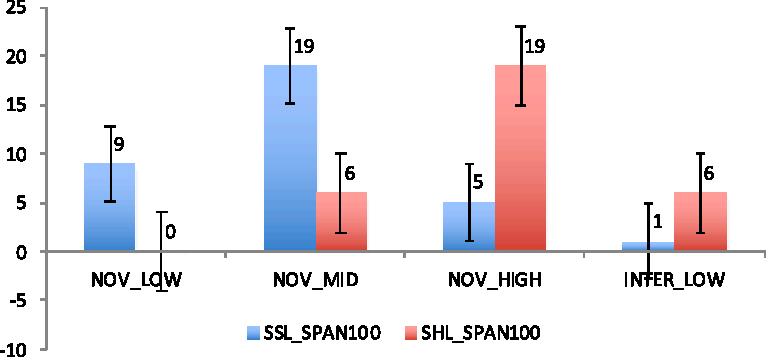
\includegraphics[width=\textwidth]{figures/Figure1-Chapter3.pdf}
\end{figure}

The horizontal axis includes sub-levels of proficiency and vertical axis relates to the number of learners who self-identified each sub-level. Error bars inform on the variability of data and indicate how precise each measurement is.

An independent samples t-test analysis was conducted to examine mean differences in the self-efficacy questionnaire measure between the first and second semester college students enrolled in the Beginning courses of the SSL and the SHL program. Most Spanish learners in Beginning-level coursework reported higher levels of confidence in the Novice to Mid-High sub-levels of speaking proficiency. In terms of differences between programs, learners enrolled in the SSL program predominantly placed themselves within the Novice-Mid continuum (mean = 1.94). SHL learners, however, expressed greater confidence than SSL learners (mean = 3.00) in their interpersonal speaking abilities, placing themselves in the Novice-High range [$t(63) = -6.19, p = 0.00$].  Additional in\-de\-pen\-dent samples t-test analysis examined mean differences in the self-efficacy questionnaire measure between the first and second semester college students enrolled in the Beginning courses of the SSL program. Second semester SSL Beginning-level learners have higher self-efficacy ratings than their first se\-mes\-ter language peers [$t(32) = -4.76,\allowbreak p = 0.00$]. However, learners in the first and second semester of the first year SHL Beginning-level courses did not differ in their perceptions of self-efficacy with regard to interpersonal speaking [$t(29) = 0.56,\allowbreak p = 0.58$].

\begin{sloppypar}
In the case of Intermediate-level coursework, the results presented in \figref{fig:3:2} portray a wider range of self-identified speaking abilities in Spanish. SSL learners mostly identified themselves as feeling capable of engaging in interpersonal speaking tasks at the Intermediate-Low level, with some considerable ratings also reported in Intermediate Mid-High. Learners in the fourth semester of the SSL Program reported higher levels of self-efficacy in the Intermediate-Mid range, as compared to their third semester peers [$t(31) = -2.81,\allowbreak p = 0.01$]. SHL learners also identified self-efficacy in interpersonal speaking at the Intermediate-Low range; however, some SHL learners also placed themselves within the Intermediate-High level. A t-test confirmed that there was no statistical difference in self-perceived ability to engage in interpersonal speaking between learners in the third and fourth semesters of Spanish in the SHL program [$t(33) = -1.35,\allowbreak p = 0.19$].
\end{sloppypar}

\begin{figure}
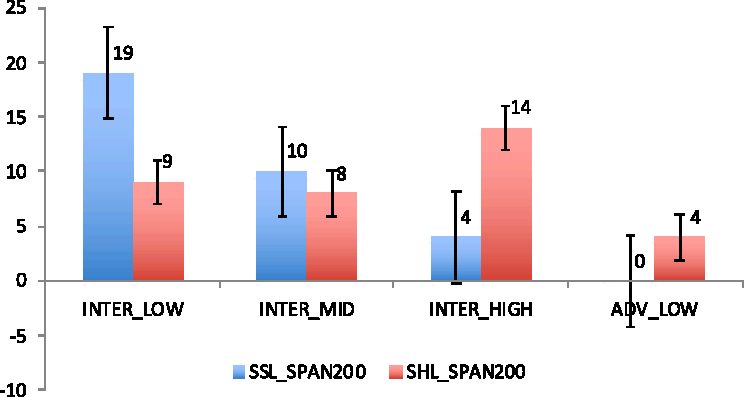
\includegraphics[width=\textwidth]{figures/Figure2-Chapter3.pdf}
\caption{Distribution of self-perceived abilities of interpersonal speaking communication in Spanish from SSL and SHL learners in Intermediate Spanish coursework (Second Year: SPAN200)}
\label{fig:3:2}
\end{figure}


\subsubsection{Presentational writing} We also compared results in learners’ reported self-efficacies in presentational writing across different levels of coursework within the SSL and SHL Programs. \figref{fig:3:3} summarizes the findings for learners’ self-perceptions of their presentational writing capabilities in Beginning-level Spanish coursework.

\begin{figure}
\caption{Distribution of self-perceived abilities of presentational writing communication in Spanish from SSL and SHL learners in Beginning-level Spanish coursework (First year: SPAN100)}
\label{fig:3:3}
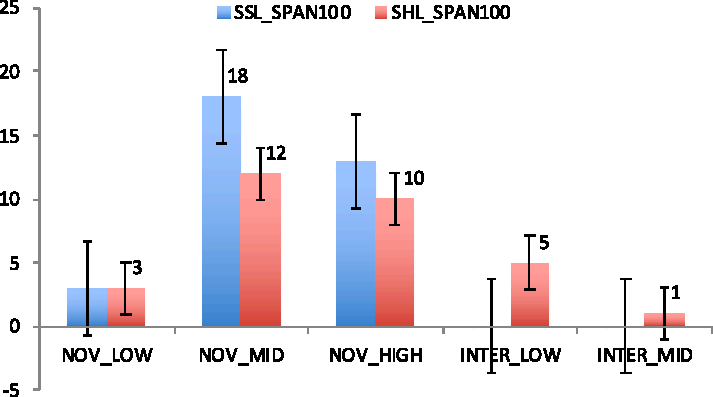
\includegraphics[width=\textwidth]{figures/Figure3-Chapter3.pdf}
\end{figure}




Overall results indicate that learners in SHL Beginning-level coursework have higher ratings of self-efficacy in presentational writing, as compared to their SSL peers [$t(63) = -2.42, p = 0.02$]. As shown in \figref{fig:3:3}, the only sub-level of proficiency that did not exhibit overlapping error bars was the Novice-Mid range. The absence of this overlap indicates that more learners in Beginning-level SSL courses exhibited higher levels of reported self-efficacies in presentational writing than their SHL Beginning-level peers.

Independent t-tests between two courses in a given program did not yield significant differences. Learners in the first and second semester of SSL identified a similar sub-level of proficiency in Spanish presentational writing [$t(32) = 0.77, p = 0.45$]. In the case of SHL Beginning (first year- semester I and II), learners in the first and second semester did not differ either in their self-perceived abilities in Spanish presentational writing [$t(29) = -0.89, p= 0.38$]. In summary, learners in first year courses in both programs perceived themselves as capable of performing tasks with a similar degree of confidence in presentational writing.

In terms of Intermediate-level coursework, there was an overall effect of similarity between SSL and SHL in Intermediate-level coursework with regard to Spanish presentational writing capabilities [$t(66) = -1.11, p = 0.27$] with the majority of learners, independently of language program, rating themselves as capable of performing at the Intermediate-Low sub-level of proficiency (\figref{fig:3:4}). When comparing third or fourth semesters of each program, there were no significant differences between self-efficacy in presentational writing among learners in the third or fourth semester in the SSL program [$t(3) = 1.02, p = 0.32$]. A similar effect was found among learners in SHL Intermediate (second year) coursework in such a way that ratings of self-efficacy did not differ among learners in third and fourth semesters in the SHL Intermediate program [$t(33) = -0.82, p = 0.42$].

\begin{figure}
\caption{Distribution of self-perceived abilities of presentational writing communication in Spanish from SSL and SHL learners in Intermediate Spanish coursework (Second year: SPAN200)}
\label{fig:3:4}
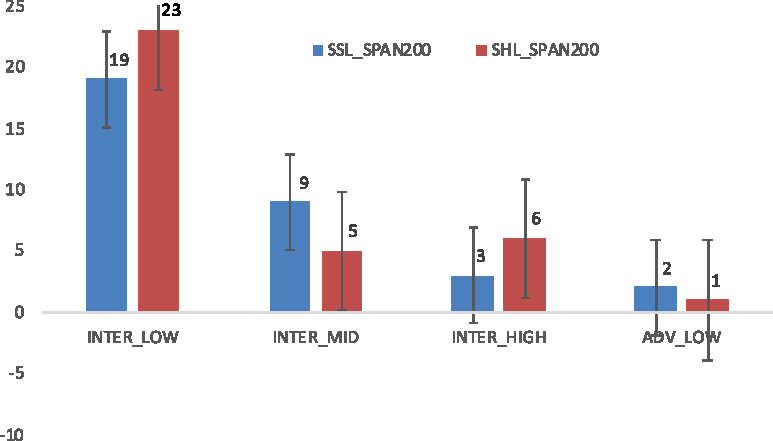
\includegraphics[width=\textwidth]{figures/Figure4-Chapter3.pdf}
\end{figure}




A snapshot of variability of ratings among learners is presented in \tabref{tab:3:2} with four 100\% stacked bar graphs that represent each language program, levels of coursework and modes of communication. There are four semesters in First and Second Year General Education coursework: 1) SPAN101 and SPAN111 = Semester I in Beginning Spanish, First year in SSL and SHL Programs, respectively; 2) SPAN102 and SPAN112 = Semester II in Beginning Spanish First year in SSL and SHL; 3) SPAN201 and SPAN211 = Semester I in Intermediate Spanish Second year in SSL and SHL; and 4) SPAN202 and SPAN212 = Semester II in Intermediate Spanish Second year in SSL and SHL.

The SSL program portrays a clearer path in terms of confidence growth, as indicated by the three colors represented in the figure for interpersonal speaking abilities. Learners in their first semester (blue) initialize rating themselves as Nov-Low/Nov-Mid and continue in their coursework by feeling more capable of engaging in interpersonal speaking activities. Throughout the sequence of SSL courses, either a monochromatic bar or a binary colored bar represents the majority of the learners, indicating that variability occurred within two proximate courses (first and second or second and third) and within two sub-levels of proficiency. However, the color sequence in the SHL figure is not as clear as the SSL one in such a way that learners in the first, second, third and fourth semester rated themselves in Intermediate-Low sub-level of proficiency. A similar scenario appears for self-efficacy ratings in the presentational writing mode of communication where a single or two colors are representative of two approximate courses or sub-levels of proficiency in the SSL Program but a wider array of perceptions is plotted throughout the different levels of coursework in the SHL program.

\begin{table}
\caption{Vignette of language proficiency trajectory of learners’ self-efficacy reported abilities based on different modes of communication and language programs throughout a sequence of four Spanish language coursework}
\label{tab:3:2}


\begin{tabularx}{\textwidth}{QQ}
\lsptoprule
\multicolumn{2}{c}{Mode of Communication: Interpersonal Speaking}\\
\midrule
\multicolumn{1}{c}{{ Spanish Second Language Program (SSL)} } & { Spanish Heritage Language Program (SHL)} \\
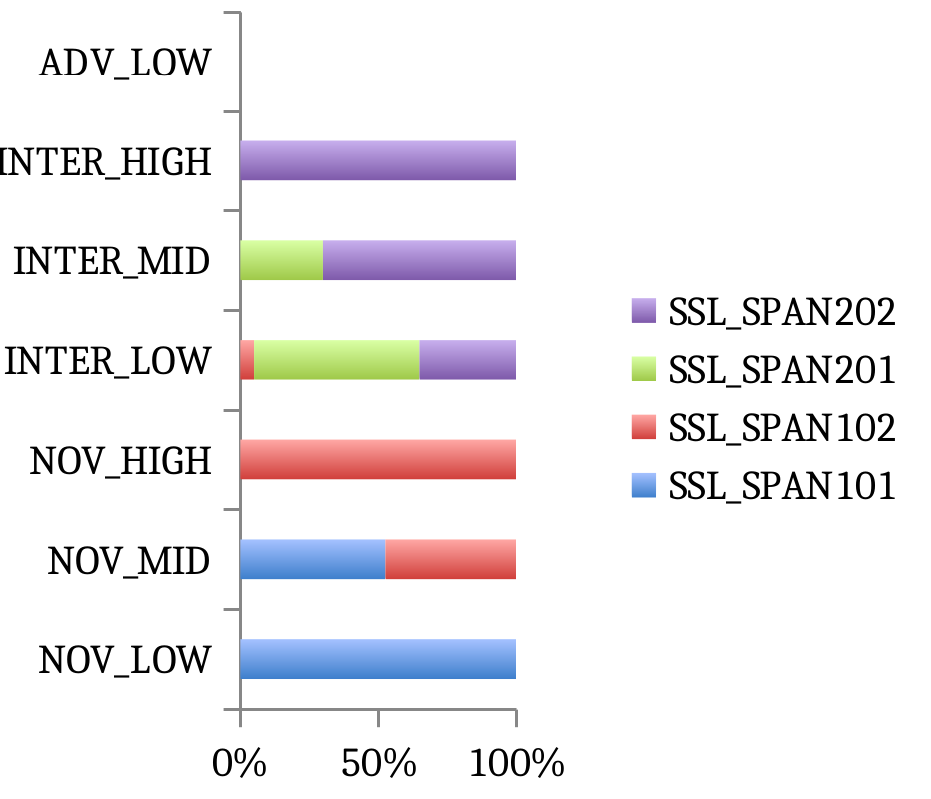
\includegraphics[width=5cm]{figures/rivera-tab-2a.png} & 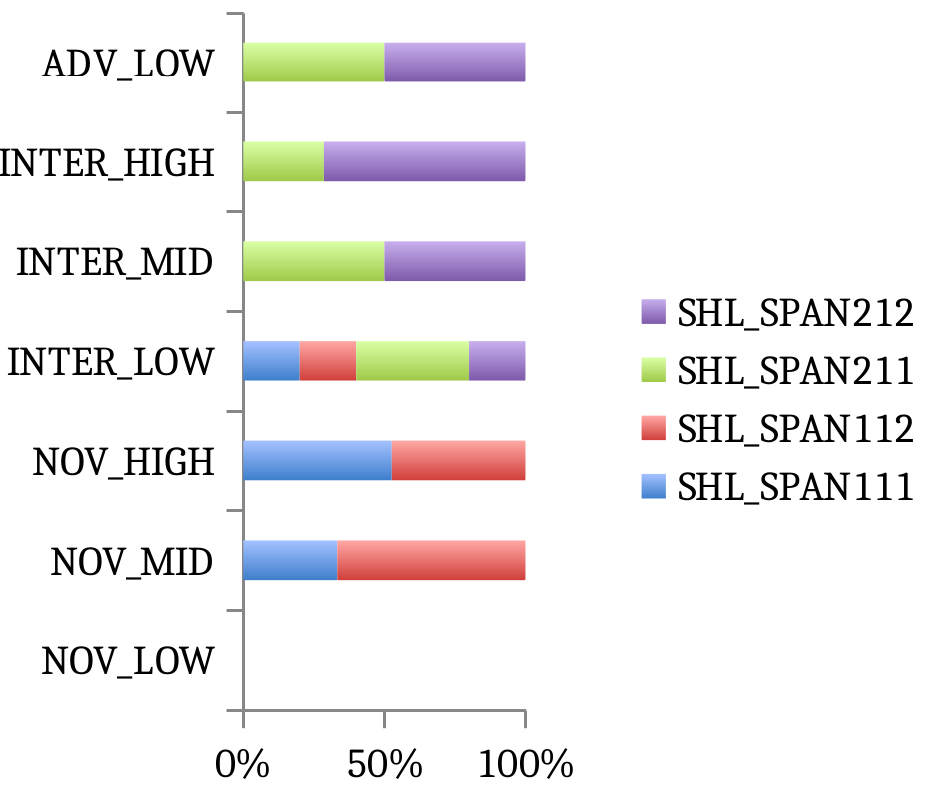
\includegraphics[width=5cm]{figures/rivera-tab-2b.png} \\
\midrule
\multicolumn{2}{c}{Mode of Communication: Presentational Writing}\\
\midrule
\multicolumn{1}{c}{SSL Program} & { SHL Program} \\
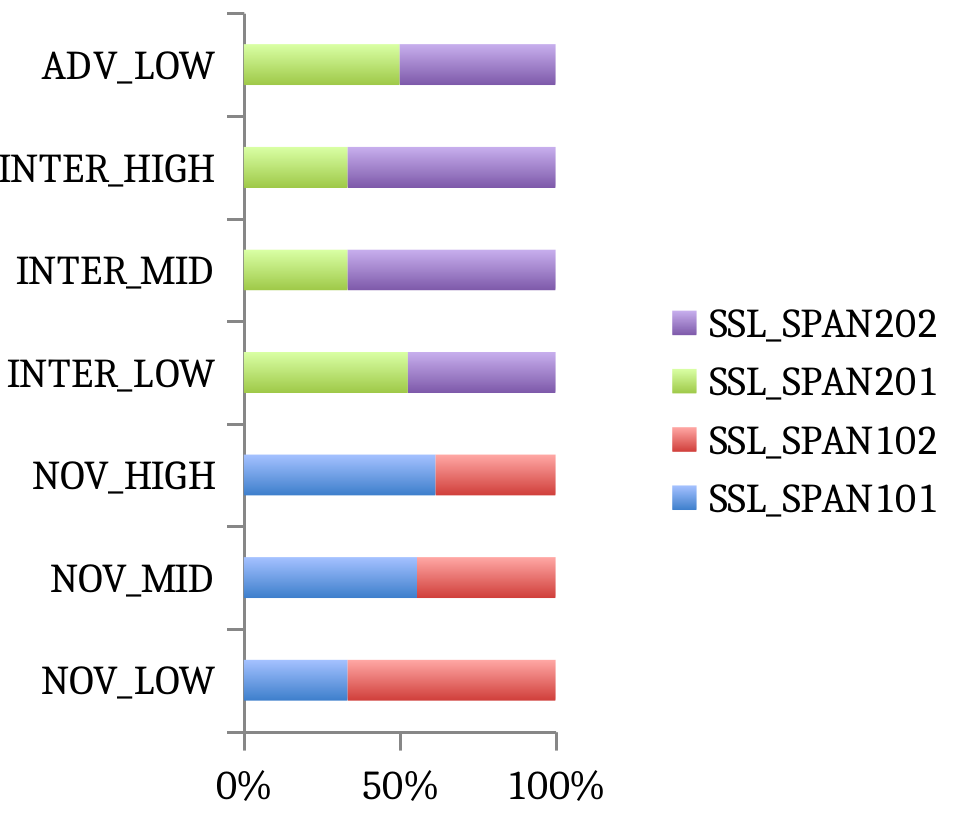
\includegraphics[width=5cm]{figures/rivera-tab-2c.png} & 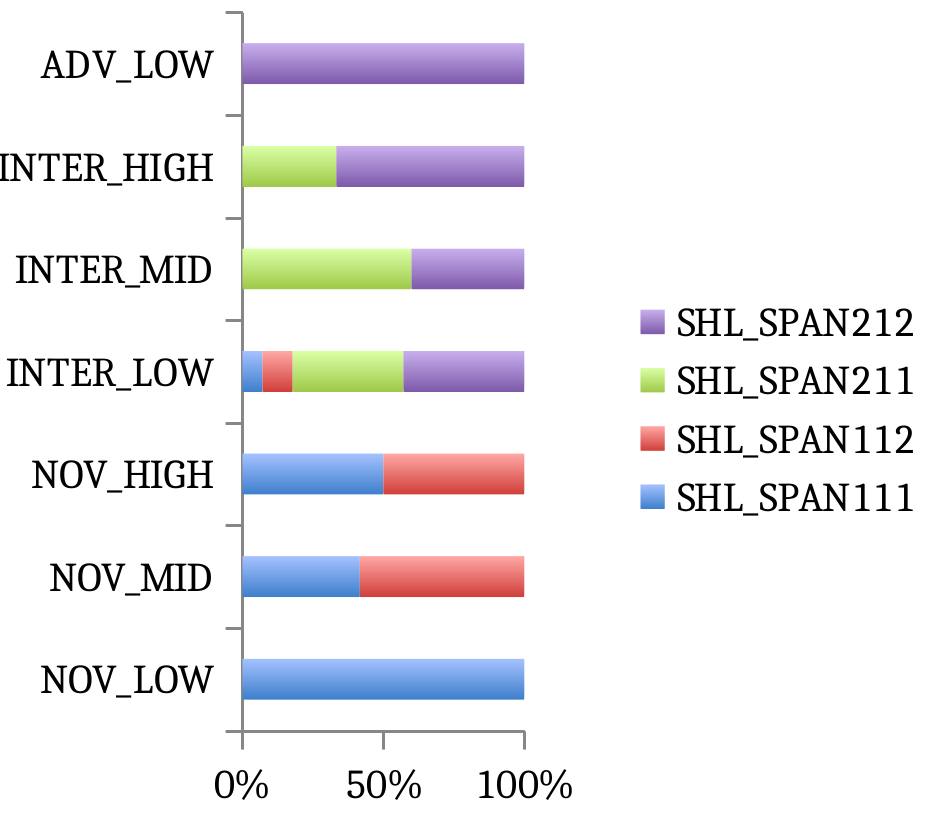
\includegraphics[width=5cm]{figures/rivera-tab-2d.png} \\
\lspbottomrule
\end{tabularx}
\end{table}



\subsection{RQ\#2: Correlation between learners’ perceptions of self-efficacy and course objectives}

\begin{table}
\small
\caption{Comparison between self-perceived abilities in speaking and writing and expected ACTFL sub-level of proficiency in course objectives determined by student learning outcomes (SLOs)}
\label{tab:3:3}
\begin{tabularx}{\textwidth}{Q@{~~}Q@{~~}QQQ}
\lsptoprule
& SSL Beginning (1st year) coursework & SHL Beginning (1st year) coursework & SSL Intermediate (2nd year) coursework & SHL Intermediate (2nd year) coursework \\
\midrule
Course SLOs

(ACTFL performance descriptors) & Novice Mid & Novice High (ACTFL equivalency) & {Intermediate High} & {Advanced Low}

 (ACTFL equivalency)\\
 \tablevspace

Self-perceptions

From \textit{Can-Do Statements} & Novice Mid (interpersonal speaking and presentational writing) & {Novice High}

{(interpersonal speaking)}

 \& Novice Mid

 (presentational writing) & {Intermediate Low}

 (interpersonal speaking and presentational writing) & {Intermediate Low}

 (interpersonal speaking and presentational writing)\\
\lspbottomrule
\end{tabularx}
\end{table}

Upon data analysis, learners’ self-efficacy ratings for interpersonal speaking and presentational writing tasks were compared across respective Spanish courses. The data served as an indirect measure of assessment on how learners’ perceived capabilities aligned with specific Student Learning Outcomes (SLOs) identified by instructors at the beginning of each course. The information presented in the first row of \tabref{tab:3:3} above outlines the different expectations of sub-levels of proficiency per course within each program. It is important to note that the SLOs for the SHL program are not necessarily aligned with ACTFL performance descriptors for different levels of proficiency. In order to compare and contrast our findings, we identified ACTFL equivalencies for SLOs in all courses of SHL program. As we see in the second row of \tabref{tab:3:3}, learners’ self-perceptions match with programmatic “expected” SLOs in Beginning coursework of both SSL and SHL programs in speaking and writing. However, the Intermediate coursework expectations and self-perceived abilities of language proficiency in interpersonal speaking and presentational writing do not match. More specifically, the distance between an expected outcome of language proficiency and self-efficacy ratings is considerable in the case of learners in the Intermediate-level Spanish coursework in the SHL program (Advanced Low vs. Intermediate Low). On a holistic view, the results confirm a direct alignment of course objectives and learners’ perceptions of self-efficacies in the Beginning-level courses in both programs.

\subsection{RQ\#3: Inclusion of \textit{Can-Do Statements} as self-efficacy tool in daily classroom activities?}

In order to answer the third research question, we propose a sample of a lesson plan that incorporates \textit{Can-Do Statements} in daily language classroom activities in an Intermediate Spanish Language course for SSL and SHL curriculum. Although the proposed instructional lesson plan has been implemented in a Latinx-serving institution in the U.S. Southwest region, it exemplifies how the exploration of current global issues, such as social justice, can be aligned with ACTFL \textit{Can-Do Statements} and applied to broader language learning contexts and classrooms where mixed language learner profiles are represented. Through this lens, the lesson plan instills a sense of awareness regarding cultural and linguistic differences, while promoting social justice in the classroom. The selected reading for the following lesson plan is \textit{La Travesía de Enrique} [Enrique’s Journey] by journalist Sonia Nazario, as the content is directly related to immigration issues. The novel addresses the reality of South American people who are leaving their countries behind for a better life in the U.S. As such, the reading is reflective of the numerous stories of Latinx communities coming to the U.S., stories to which many learners can readily recognize and relate. For instance, some learners may have familial immigration histories that are similar to those evidenced in the novel, while others may associate the story’s events with immigration issues that they see in the news and other media. The events explored in \textit{La Travesía de Enrique} therefore serve as the framework for the lesson plan. The lesson plan itself facilitates conversations about current political issues that allow students to reflect and critically think on patterns of inequality, discrimination, and injustice. It also empowers learners to examine and question situations that they deem unfair in their lives or the lives around them.

With the focus of the lesson established, the \textit{Can-Do Statements} were then embedded as a pedagogical tool to measure how learners rated their abilities in the different language areas. Important to note is that the \textit{Can-Do Statements} included in the present study were also utilized in SSL courses as a continuous, semester-long self-evaluation assessment. The overall design of the lesson plan thus exemplifies how \textit{Can-Do Statements} can be interwoven to support the exploration of a topic that encompasses global and community issues, thereby establishing inclusivity for both L2 and HL learners.

While data from the \textit{Can-Do Statements} informed the proposed design of lesson plan for learners in Intermediate L2 Spanish program, this theme can also be adapted for HLLs (see \tabref{tab:3:5} for details). The \textit{Can-Do Statements} checklists used in the present study were distributed before a lesson plan and were implemented and returned to learners with the appropriate feedback following the parameters of \textit{Linguafolio} and identified ACTFL performance descriptors for the activities and the course.

For this specific sample, we designed the activities based on ACTFL performance descriptors for Advanced Low level of proficiency. Although the ACTFL proficiency level identified in the course (cf. list of student learning outcomes) was Intermediate High, classroom activities have been designed with Advanced Low performance descriptors following Krashen’s $i + 1$ comprehensible input principle (\citealt{Krashen1982,Krashen1985}). As such, comprehensible input is that input which is slightly beyond the current level of competence of a language learner. If \textit{i} is the language learner’s current level of competence in the target language, $i + 1$ is the next immediate step along the development continuum.~In this particular course, course activities have been designed for Advanced Low level of proficiency as the next immediate sub-level following the identified Intermediate High expected level of proficiency in the course.

\tabref{tab:3:4} provides a summary of the student learning outcomes identified for different activities based on speaking and writing language skills. A series of \textit{Can-Do Statements} portrayed in the table correspond to each learning outcomes for speaking and writing. SAL refers to Speaking Advanced Low learning outcomes to be assessed and the number refers to their place in the list. WAL stands for Writing Advanced Low and the number equally refers to which of the \textit{Can-Do Statements} from the list we are referring to. The \textit{Can-Do Statements} have been adapted to activities that 1) reflect on immigration issues in the U.S.; 2) identify key points and reframe them by using learners' own words; and 3) compare primary sources and connect them to lived experiences. In the different activities, learners reflect on immigration, identify key terminology and paraphrase, compare and connect the reading with their personal experiences on the subject matter.

\begin{table}
\caption{List of \textit{Can-Do Statements} used for self-assessment in the proposed lesson plan (based on ACTFL performance descriptors at Advanced Low level of proficiency)}
\label{tab:3:4}
\begin{tabularx}{\textwidth}{QQ}
\lsptoprule
{ Speaking\newline (interpersonal communication)} & { Writing\newline  (presentational communication)} \\

\midrule

{ Advanced Low:}\medskip

SAL1.2 I can explain current issues, such as social inequality, discrimination, and immigration journey stories.\medskip

SAL1.3. I can discuss what is currently going on in borders across countries and different communities.\medskip

SAL.4. I can conduct or participate in interviews on family stories in my community. &

{ Advanced Low:}\medskip

WAL3.1 I can manage and edit an online journal, blog, or discussion forum on current issues about immigration and border issues.\medskip

WAL3.2 I can write an article about a personal story or political issues. \\

\lspbottomrule
\end{tabularx}
\parbox{\textwidth}{\footnotesize SAL = Speaking Advanced Low and WAL = Writing Advanced Low. The numbers represent the adapted Can-Do statement numbering from \textit{Linguafolio}.}
\end{table}

\textit{The lesson plan:} The design consisted of a series of activities for a Spanish intermediate-level course (fourth semester- Intermediate Spanish II). These proposed activities are not time-sensitive and can be used and adapted throughout a given instructional period. The four-day lesson plan described below is not time-bound, as it could be completed in a one to two-week frame or the time the instructor considers appropriate depending on their syllabus and course objectives. Furthermore, each activity is aligned with specific \textit{Can-Do Statements} identified in \tabref{tab:3:4} and is connected to the specific mode of communication (i.e. interpersonal, presentational or interpretive) and the particular instructional objective. All the activities in the present lesson plan may be differentiated for L2 and HLLs.

For this lesson plan, we have identified Advanced Low performance descriptors for the activities with the understanding that instructors must remain cognizant of their learners’ linguistic capabilities and align the ACTFL proficiency guidelines with the specific learning needs of their student population (see \tabref{tab:3:5}). To be consistent with the results presented for RQ 1 and 2, the current lesson plan focuses on self-assessment of speaking and writing as these were the language skills participants in the study reported as feeling less confident in.

\begin{table}
\footnotesize
\caption{Proposal of activities for a lesson plan that integrates learners’ self-assessment (via \textit{Can-Do Statements}) in an Intermediate-level Spanish course for L2 and HL learners.}
\label{tab:3:5}
\begin{tabularx}{\textwidth}{p{2cm}Q}

\lsptoprule

\multicolumn{2}{p{.95\textwidth}}{
    \textbf{Sample Lesson Plan}

    Lesson Objectives:

    1. Reflect on immigration issues in Latinx communities in Latin America and the U.S. at the local, regional and national level

    2. Identify key points and reframe them using your own words

    3. Compare primary sources and connect them to lived experiences

    4. Reflect on equity, diversity and inclusion practices in our language classroom in relationship with Latinx communities
}
\\
\midrule
Presentational & \textbf{Pre-} \textbf{(Brainstorming)} \textbf{Activity}\newline
Blog (written): Reflect on immigration in the U.S.: What do you know? What would you like to know? Share your responses with your peers.

Can-Do Statement: WAL3.1

\textit{Differentiation for SHL: How does it relate to your family history?}\\

\midrule
Interpretative, interpersonal and presentational & \textbf{Reading} \textbf{in} \textbf{class} \textbf{Activity}
\begin{itemize}[leftmargin=*]
\setlength{\itemsep}{0pt}
\item Students are recommended to read the designated chapter from Enrique’s Journey assigned in a previous class to become familiar with new vocabulary terminology.
\item An excerpt of the text is selected by the instructor and will be divided in sections.
\item Each group (two students) is assigned a section. Sections are dispersed on poster paper around the classroom.
\item Students decide who is in charge of writing and who is in charge of paraphrasing.
\item One or two students read the section and then return to report what they understood to the student taking notes. They can write notes on vocabulary that they do not know. The report from the group takes the form of a written summary of what they understood from the dictation.
\item Students switch roles to 1) provide as much detail as possible in the written summary and 2) to have an opportunity to practice interpretive and interpersonal skills
\item Students extract information and will present what they read from the excerpts from Enrique's Journey presented in the posters.
\item Classroom engages in a discussion related to Enrique’s story and related social justice issues that evolve from the reading: students first discuss the story via a jigsaw where they share their ideas and opinions on what they understood from the reading. The final discussion goes beyond the reading per se and extends on similar stories of immigration based on social justice, equity, diversity and inclusion.
\end{itemize}
Can-Do Statement: SAL1.2 and SAL1.3\\
\midrule
\end{tabularx}
\end{table}
\begin{table}%cont
\footnotesize
\begin{tabularx}{\textwidth}{p{2cm}Q}
\midrule
\raggedright
Interpretative,
and presentational & \textbf{Post-Reading} \textbf{Activity}

Video recording:  Students will record a video in which they discuss a newspaper article on immigration of Latinx community in Latin America or/and the U.S. They will compare this information with what they read in class. They will also answer why they believe it is important to know about this topic.

Can-Do Statement: SAL1.3\\
\raggedright
Interpretative,
and Interpersonal &
\textit{Differentiation for SHL: Audio recording: Students interview a family or community member regarding their experience as an immigrant in the US. They will record this conversation and respond to the question: Why is this topic important in my community? What would you like others to know about your community?}

\textit{Can-Do Statement: SAL4}\\

\midrule
\raggedright
Presentational,
interpersonal  & \textbf{Final} \textbf{Closing} \textbf{Activity}

Blog 2 (written): After reading to peers’ responses from posts in Blog 1, students respond to their own first entry (blog 1): What have you learned about immigration and personal stories? How has all this info impacted the way you think about discrimination, injustice and inequality after being exposed to \textit{Enrique's Journey} and other related stories?  In your answer, use evidence from the book and newspaper. This final activity opens a safe discussion space for students to reflect on the value of diversity, inclusion and equity in Latin America and the U.S.

Can-Do Statement: WAL3.1, WAL3.2.

\textit{Differentiation for SHL: Use evidence from interview from previous SHL activity and compare to the book.}

Can-Do Statements: WAL3.1, WAL3.2, SAL1.2, SAL1.3, SAL4\\
\lspbottomrule
\end{tabularx}
\end{table}


The proposed lesson plan in \tabref{tab:3:5} includes collaborative learning-based activities that are focused on Latin America-U.S. immigration issues. By engaging in these activities, students learn about aspects of immigration and connect this understanding to the personal experiences of Latin American immigrants. To prepare for the \textit{Final in-class discussion}, instructors may start with a baseline \textit{Pre-reflection activity} that encourages students to identify what they believe they understand about immigration, as well as highlight potential areas of new information. This preliminary activity encourages students to think critically on why and how individuals and/or families immigrate.\largerpage

During \textit{Reading in-class activities}, students identify key concepts and reflect on the experiences of immigrant children by reading an excerpt of \textit{Enrique's Journey}. They are to analyze the reading, identifying how the content addresses issues of equity, diversity and inclusion. For the \textit{Post-Reading video recording activity}, students are encouraged to use other sources of information and engage in an ethical debate about the nature and dangers of immigration. Students may discuss how \textit{Enrique’s Journey} parallels reality by referencing authentic newspaper articles of their choice. This activity subsequently allows students to become agents of their own knowledge.\largerpage

In the \textit{Closing activity}, students will discuss how their previous understanding on the topic has evolved from the preliminary activity (Blog 1). This final activity facilitates personal learning via the ongoing process of reflection and connection to human experiences and the realities of our globalized world. Teachers can tailor the lesson plan for L2 and HLLs by incorporating the questions in italics in the table and encouraging students to make personal connections to their own communities.

Throughout the sequence of proposed activities, students reflect upon their learning and monitor their own language development by means of the \textit{Can-Do Statements} and self-assessment. Each section and activity thus measures to what extent learners feel comfortable to talk and write about diversity, equity, and inclusion as a framework for understanding Latinx immigration and border issues in the U.S. The goal of this proposed lesson plan was to provide language instructors with some direction on how to use self-assessment monitoring techniques to shape learners’ perceptions of their language capabilities. As learners’ metacognitive knowledge and learning strategies evolve, learners are better able to plan, carry out, and assess their own learning (\citealt{CouncilofEurope2002}; \citealt{LittlePerclova2001}).


\section{Discussion}\largerpage[2]

One of the most challenging areas in language teaching concerns the scaffolding of student learning to transition from colloquial, everyday language use to a decontextualized, academic register. \citet{Cummins1979} described this process within English language learners as the development of Basic Interpersonal Communication Skills (BICS) to advance toward Cognitive Academic Language Proficiency (CALP). For L2 learners, the development of BICS to CALP communication skills follows a rather predictable, linear pattern (\citealt{Montrul2011b}). As evidenced in this study, however, such a linear trajectory does not necessarily exist for HLLs.

By virtue of their natural exposure to the language, HLLs often possess a wide array of linguistic skills and vocabulary, which typically manifest in a broader BICS communicative range than L2 learners. As a result, beginning HLLs may feel more confident with speaking the target language in social situations. This confidence may fluctuate, however, when HLLs are required to understand advanced grammatical concepts and apply this knowledge to speak or write in an academic register (\citealt{Beaudrie2009}; \citealt{Carreira2003}; \citealt{Correa2011}; \citealt{Montrul2011}; \citealt{Zyzik2016}). Given this variability in HLL self-efficacy, it is essential that self-reported assessments, such as the \textit{Can-Do Statements}, serve as a flexible document through which instructors can better align their practices to the needs of their student population (\citealt{CoxWinke2018}: 108).

The present study thus examined four levels of coursework to determine the development of BICS throughout Beginning and Intermediate levels. Of particular interest was exploring the bridging of BICS and CALP skills within the fourth semester course, Intermediate Spanish II. To explain, beginning-level coursework provides learners with opportunities, such as role-play exchanges, to learn the target language for sophisticated, social interactions. Knowledge of BICS is therefore important to help learners feel comfortable speaking and writing the language in socially and culturally appropriate contexts. On the other hand, knowledge of CALP is essential for academic success and for critical thinking.

The fourth semester of the last intermediate language course is therefore a pedagogically operationalized space where BICS and CALP can be included in cognitively stimulating and socially meaningful activities. In this regard, the incorporation of self-assessment of output language skills can help learners reflect upon their own language learning and identity in a more globalized society where different cultures and linguistic profiles are equitably represented. The set of classroom activities proposed in this study were thus designed with \textit{equity} as a core principle.

Students enrolled in the Beginning and Intermediate courses in the SSL program developed their speaking and writing skills in Spanish through authentic media-based readings that focused on the social and political realities of Central American immigration to the United States. The inclusion of culturally representative readings, such as \textit{Enrique’s journey}, makes a case for a responsive pedagogy that is sensitive to the social realities of the Spanish language and culture, while also having students reflect on their self-efficacy. As such, the sample lesson plan provided in this chapter facilitates and enhances learner self-confidence through activities that promote a sense of belonging through the Latinx community, and validation of self-worth and cultural and linguistic identity.

Affirmative \textit{Can-Do Statements} can contribute to the validation of self-worth and learner identity, as they intrinsically make learners reflect where they are in the process of learning of Spanish. As previously mentioned, self-assessment stimulates learners’ autonomy and their language development. Through the implementation of self-assessment checklists identified in the \textit{Can-Do Statements}, learners can develop specific skills such as monitoring, planning, improving and evaluating their own learning. Additionally, the development of these skills pre\-sents advantages that are valuable to the learners beyond the classroom setting. For instance, self-assessment helps learners to develop meta-cognitive skills that can be applied later on in their lives to evaluate their professional performance. It also enhances self-awareness through reflective practice. Likewise, by exercising self-assessment, language learners improve their critical reviewing skills facilitating them to be more objective of their own learning and others. Last but not the least, self-assessment enhances learners’ agency by enriching their own learning through meaningful reflection and evaluation. As such, self-assessment is a valuable, alternative form of assessment to traditional assessments as long as students have been guided and trained on how to self-evaluate their own learning.

The empirical results reported herein should be considered in the light of some limitations. Foremost, the present study did not include the instructors’ perceptions regarding the capabilities of their students, and as such, there is no comparative data that explores the learner’s self-perceived capabilities of Spanish speaking and writing with their instructors’ observations. Another variable that was not investigated in this study was how language anxiety influenced learners’ self-reported data. The role of anxiety in relation to different language profiles, such as second/heritage language learning, should subsequently be explored in the future. Additionally, communicative anxiety when writing and/or speaking any languages and the age of acquisition are other important factors to examine (\citealt{DewaeleFurnham2008}; \citealt{SparksGanschow1991}). Lastly, this study only focused on speaking and writing skills. Further research should therefore examine learners’ self-perceived capabilities of language learning in other skills and competencies, such as listening, reading and intercultural competence; to see if self-efficacy traits are similar to or different from those found in speaking and writing.


\section{{Conclusion}}

\begin{sloppypar}
This study contributes to existing research on the exploration of self-efficacy within the context of higher education language learning classrooms. By examining how participants in two Spanish language programs self-assessed their abilities in two domains, written and spoken, the authors were able to design a pedagogical tool that allowed learners to advance their level of proficiency through inclusive and diverse classroom activities. Overall, the findings underscore the importance of measuring learners’ perceived linguistic capabilities as a method to inform classroom instruction. Specifically, intermediate language coursework must incorporate tasks that require learners to routinely measure their self-efficacy. This increased awareness of one’s linguistic capabilities is especially critical in mixed classrooms, where the differing levels of proficiency, diverse learner profiles, and self-efficacies can exacerbate learners’ feelings of anxiety. By implementing an instructive design based on student self-efficacies and curriculum objectives, instructors are able to 1) help learners positively identify their language skill sets; and 2) better plan activities that encourage learners to build their self-efficacies in oral and written skills. This insight can then inform best practices that integrate language awareness and self-assessment through the lens of social justice. Alternative assessments that are based on self-efficacy driven \textit{Can-Do Statements} can thus bring into language classrooms current events and cultural manifestations that are meaningful within Latinx communities.
\end{sloppypar}

In conclusion, the findings and proposed curriculum in the present study call for a more contextualized approach to language instruction and planning that takes into consideration the learning outcomes that the students’ themselves identify as goals to their success. By integrating learners’ voices on self-perceived capabilities into language coursework, instructors may draw on this kind of data as a baseline for the development of a more reliable set of course learning outcomes in both cross-sectional and vertical curriculum alignment.

\sloppy
\printbibliography[heading=subbibliography,notkeyword=this]

\end{document}
